% $Id: objectmappingprefs.tex 7846 2009-02-24 13:51:53Z alexandra $
% Local Variables:
% ispell-check-comments: nil
% Local IspellDict: american
% End:
% --------------------------------------------------------
% User documentation
% copyright by BREDEX GmbH 2005
% --------------------------------------------------------
\index{Preferences!Object Mapping}
\index{Object Mapping!Preferences}
\index{Heuristic}
\label{objectprefs}

\begin{itemize}
\item To edit the object mapping preferences, open:\\
\bxmenu{Window}{Preferences}{}\\
and select \bxcaption{Object Mapping} from the left-hand side.
\item In the dialog which appears (see \bxfigref{objectmappingpref}), you can:
\begin{description}
\item[Show number of child nodes:]{activating this option shows the number of items contained in each category. If the \gdomeditor{} is open, you will have to close it and reopen it for the changes to take effect.}
\item [Edit the key combination for collecting components:]{You can choose a key combination that is not already taken in your \gdaut{}. You can also specify that clicks should be used to collect components. The key combination settings cannot be changed for iOS or HTML \gdauts{}.}
\end{description}
\end{itemize}

\begin{figure} [htbp]
\begin{center}
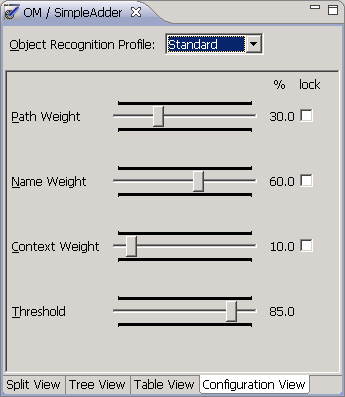
\includegraphics{Tasks/Objectmapping/PS/objectmappingpref} 
\caption{Object Mapping Preferences}
\label{objectmappingpref}
\end{center}
\end{figure}
